\documentclass{article}
\usepackage{titlesec} 
\usepackage{tikz}
\usepackage{xcolor}
\usepackage[left=1cm,right=1cm,top=1cm,bottom=1cm]{geometry}
\usepackage{fancyhdr}
\definecolor{LightBlue}{RGB}{66, 163, 251}
\definecolor{DarkBlue}{RGB}{36, 100, 176}
\definecolor{LightGray}{gray}{.94}
\definecolor{DarkGray}{gray}{.172}
\definecolor{Orange}{RGB}{229, 133, 3}
\definecolor{MediumBlue}{RGB}{38, 119, 193}
\titleformat*{\section}{\color{DarkBlue}\normalfont\bfseries\Huge}
\titleformat*{\subsection}{\color{LightBlue}\normalfont\bfseries\LARGE}
\titleformat*{\subsubsection}{\color{MediumBlue}\normalfont\bfseries\LARGE}




\begin{document}

\section{DISNEY MOVIES ANALYSIS REPORT}

\subsection{Rating distribution of Disney movies among IMDB and Rotten Tomato  }
Disney has released a total of 432 Movies since 1937 and it's  content is loved all over the world. Specially among kids.


    \begin{figure}[htp]
    \centering
       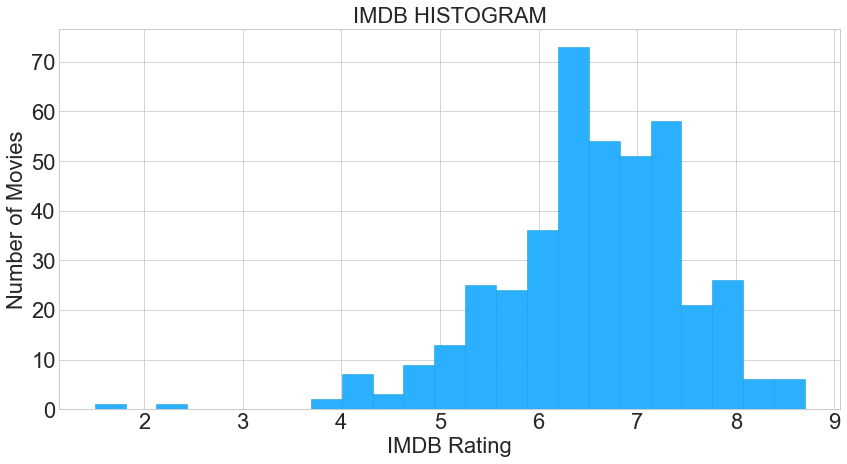
\includegraphics[width=.4\textwidth]{figures/1.png}\hfill
    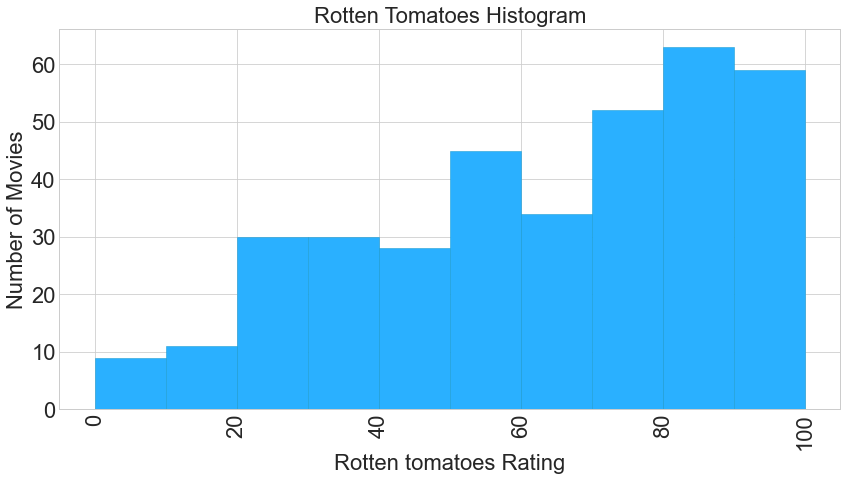
\includegraphics[width=.4\textwidth]{figures/3.png}
    \textcolor{Orange}{\textbf{\caption{Histogram Description of IMDB rating and Rotten Tomato Score}}}\label{fig:1}
    \end{figure}
    
IMDb ratings are done by viewers while on the other hand Rotten Tomatoes are based on real critics. Based on the above three histogram distribution of disney movies , We can conclude  that not all movies with Disney tag  is liked by viewers , Since most of the movie rating on IMDB  lies  in the range of 6 and 7, And a very few movies made it to IMDB Rating above 8. \newline
But on the otherhand unlike IMDB rating disney movies has performed exceptionally well in Rotten Tomato were most of the movie score  lie in the range of 80 to 100. This also means that disney movies are liked more by critics for it fresh content and amazing stories then the viewers.

  \begin{figure}[htp]
    \centering
      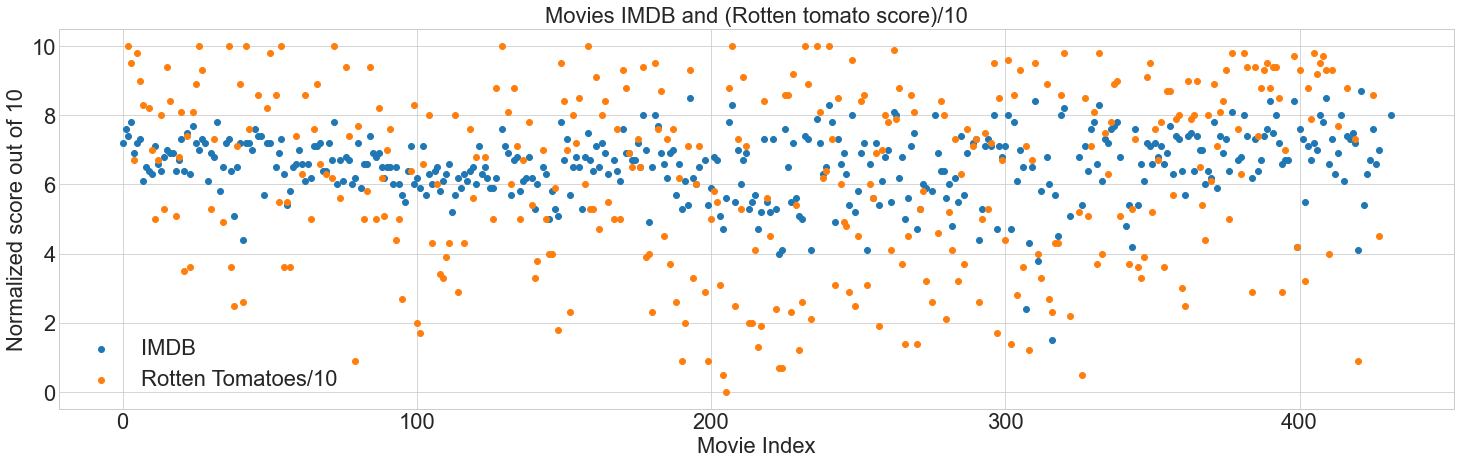
\includegraphics[width=1\textwidth]{figures/2.png}
       \centering
      \textcolor{Orange}{\textbf{\caption{Scattered Distribution of IMDB rating and Rotten Tomato Score out of 10}}}\label{fig:2}
    \end{figure}
From Figure 2 and Figure 1 we can conclude that Disney movie's IMDB rating is the range of 4 to 8 with a few exceptions while on the other hand Rotten Tomatoes Score are very much scattered in the range 0 to 100 with increasing frequency towards higher score.

\newpage


\subsubsection{Disney Movie Running Time}

\noindent\begin{minipage}{0.4\textwidth}
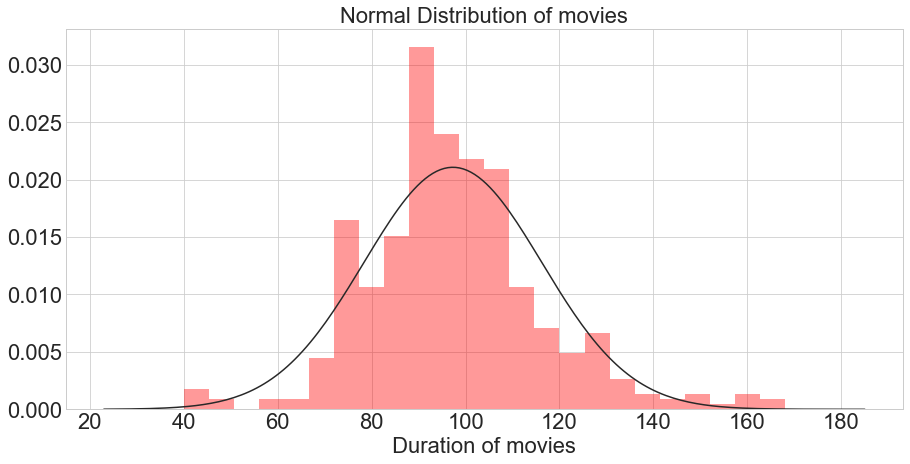
\includegraphics[width=\linewidth]{figures/8.png}
 \textcolor{Orange}{\textbf{\captionof{Fig 3: }{Normal Distribution of Movies runtime}}}
\end{minipage}%
\hfill%
\begin{minipage}{0.55\textwidth}
From The Normal Distribution of Movies Run Time in \textbf{\textcolor{Orange}{Fig 3}}  we see that most of the Disney movie have a run time of around 90 minutes.
\end{minipage}
 
\subsubsection{Disney Movie Revenue and IMDB rating}

\noindent
\begin{minipage}{0.55\textwidth}
From The Scattered Distribution in \textbf{\textcolor{Orange}{Fig 4}}  we can infer that all the low  IMDB  rated movies\textit{ ( IMDB rating less than 6 )} either have have a loss or low revenue as compared to other Disney movies with higher rating.
\end{minipage}\hfill%
\begin{minipage}{0.4\textwidth}
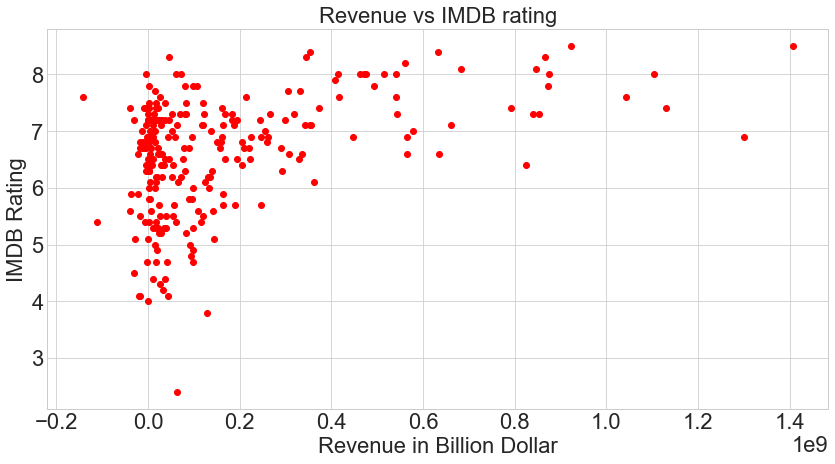
\includegraphics[width=\linewidth]{figures/13.png}
 \textcolor{Orange}{\textbf{\captionof{Fig 4: }{Scattered Distribution of Movies Revenue with IMDB rating}}}
\end{minipage}%


\subsubsection{Average IMDB rating of Disney Movies  per year}

\noindent\begin{minipage}{0.4\textwidth}
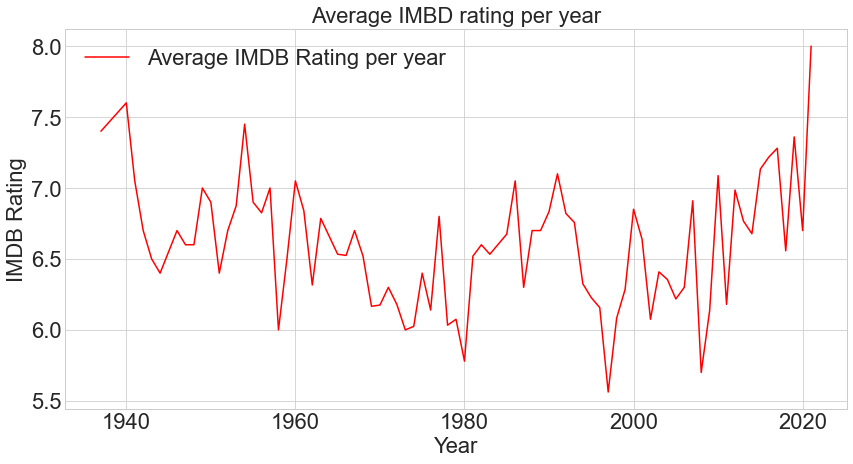
\includegraphics[width=\linewidth]{figures/14.png}
\textcolor{Orange}{\textbf{\captionof{Fig 5: }{Trend of Average IMDB rating per year}}}
\end{minipage}%
\hfill%
\begin{minipage}{0.4\textwidth}
From the Trend of average IMDB rating of movies produced in a year, we can clearly see there a downward trend from first year Disney released it's movie till 2000 although we can see a upward trend after 2000  till present Year 2021 being the highest.
\end{minipage}
\subsubsection{Disney Movie Release by Month }
\noindent
\begin{minipage}{0.55\textwidth}
Disney has launched most of it's movies in the month of January may be because of that it has launched the least number of movies in the month of December and November.
\end{minipage}\hfill%
\begin{minipage}{0.25\textwidth}
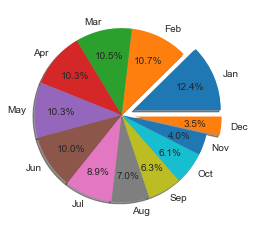
\includegraphics[width=\linewidth]{figures/5.png}
\end{minipage}%

\subsubsection{Last 20 years count of IMDB rating above and below 7.5}

\noindent\begin{minipage}{0.4\textwidth}
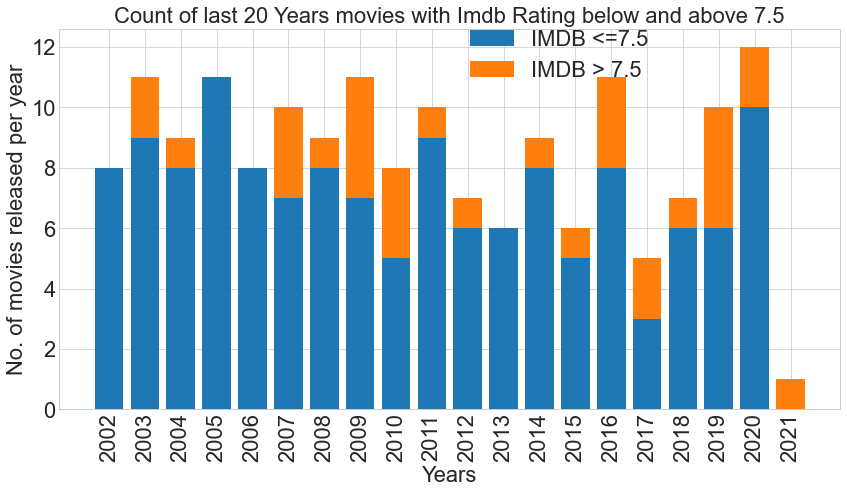
\includegraphics[width=\linewidth]{figures/17.png}
\textcolor{Orange}{\textbf{\captionof{Fig 6: }{Count of IMDB rating above and below 7.5}}}
\end{minipage}%
\hfill%
\begin{minipage}{0.55\textwidth}
Disney movies with IMDB Rating less than 7.5 is subsequently larger than  movies with rating above 7.5 , Although Disney managed to get a maximum of 4 movies in 2009 and 2019  with IMDB rating above 7.5
\end{minipage}
\subsection{Top 10 Country, Language, Director ,Producer : Disney Movies}



    \begin{figure}[htp]
    \centering
       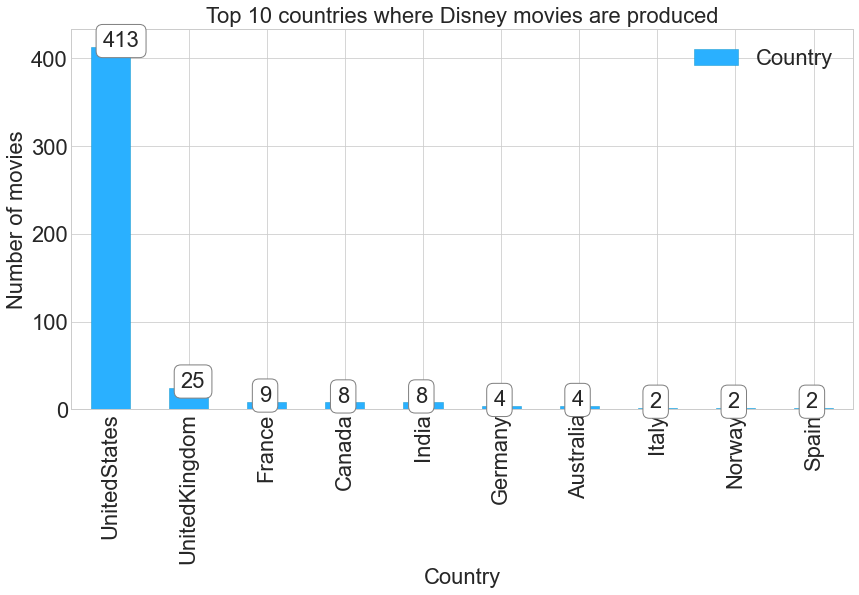
\includegraphics[width=.4\textwidth]{figures/9.png}\hfill
    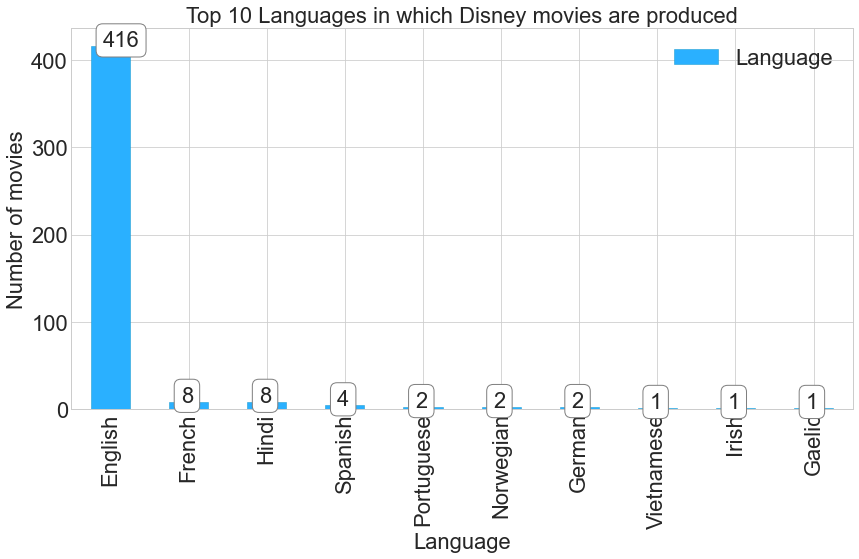
\includegraphics[width=.4\textwidth]{figures/10.png}
     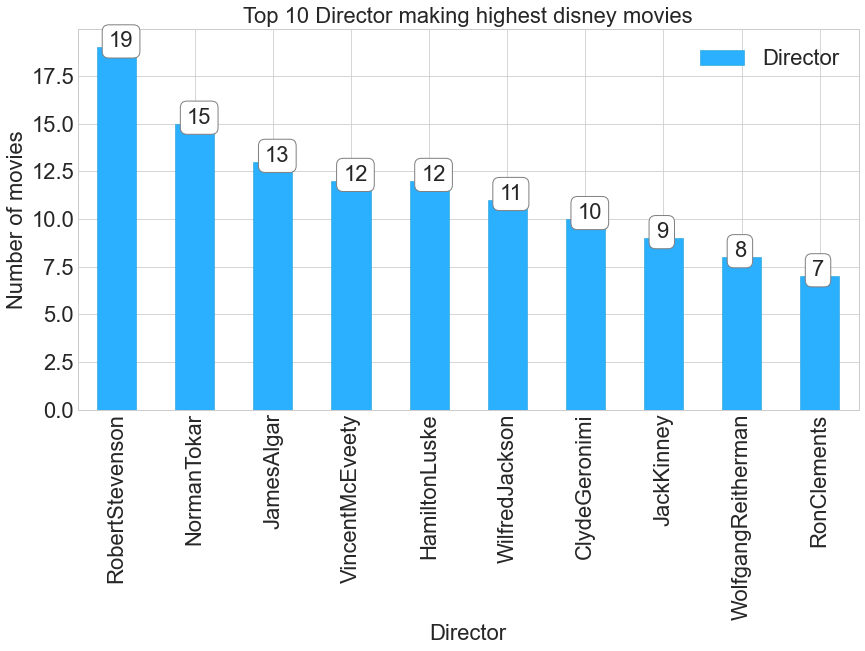
\includegraphics[width=.4\textwidth]{figures/11.png}\hfill
    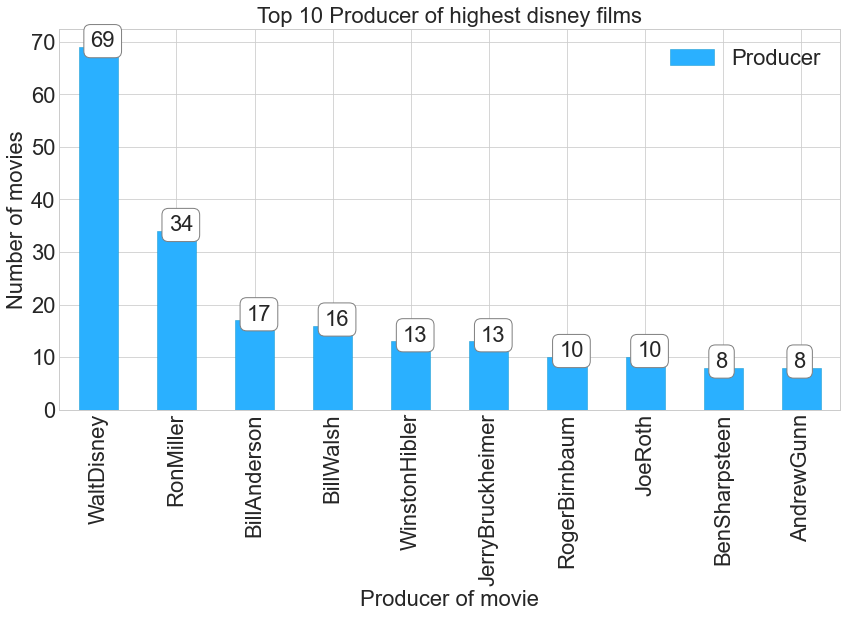
\includegraphics[width=.4\textwidth]{figures/12.png}
    \end{figure}
Most of the Disney movies are produced in United States with  English being the most popular language.\\
Robert Stevenson has directed the highest number of Disney movies and Walt Disney was the producer of most Disney moves.
\newpage

\subsection{Box Office and Budget of Top 10 and Worst 10 movies by IMDB rating }



    \begin{figure}[htp]
    \centering
       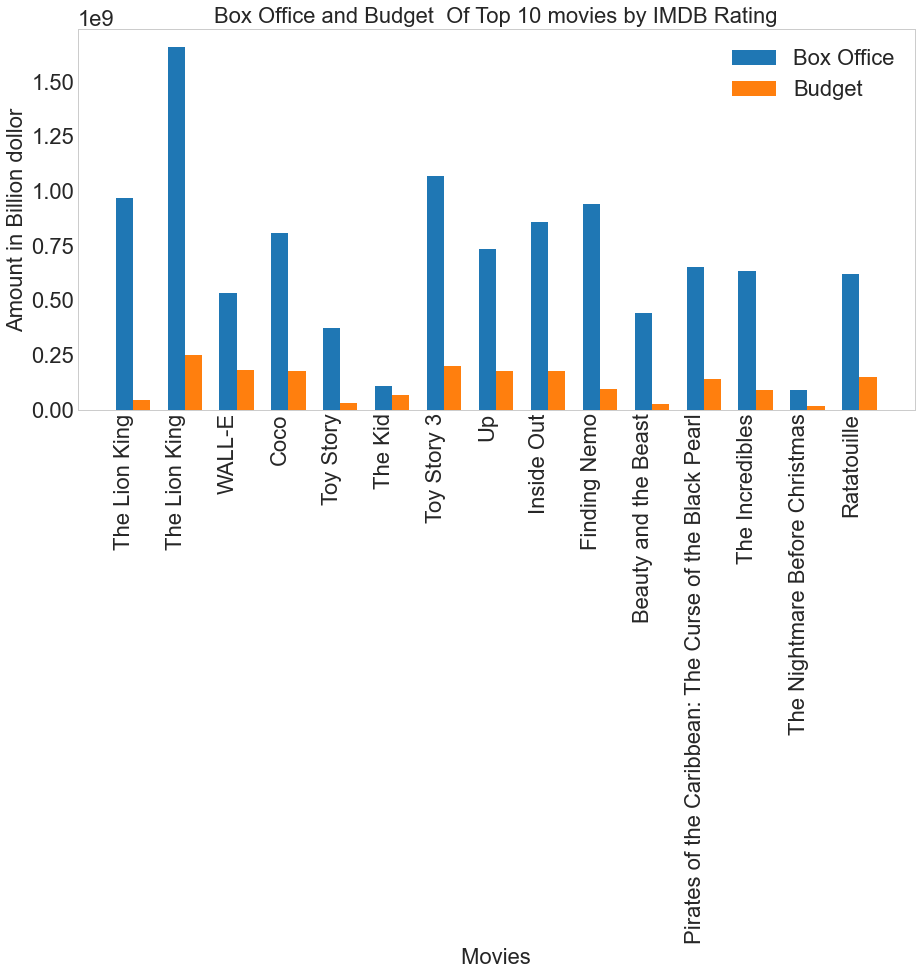
\includegraphics[width=.36\textwidth]{figures/6.png}\hfill
    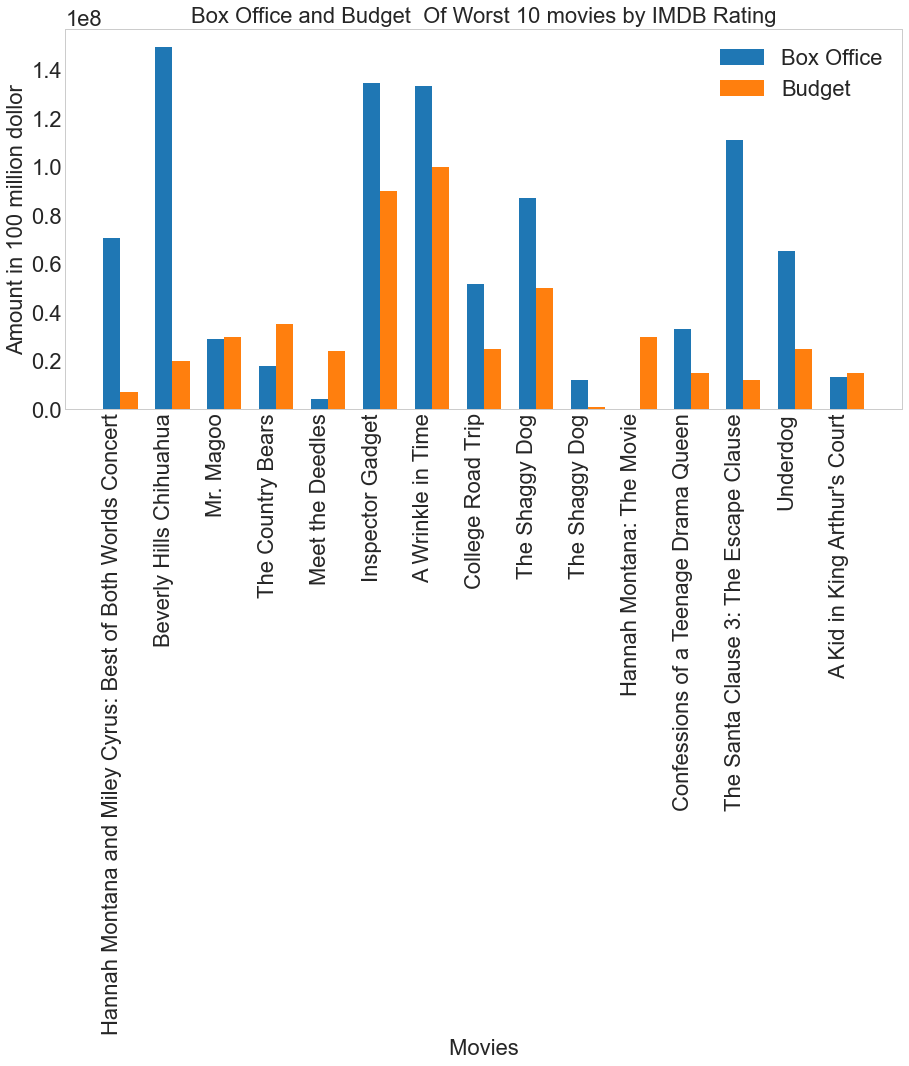
\includegraphics[width=.36\textwidth]{figures/7.png}
    
    
    \end{figure}

In the Top 10 IMDB rated movies the difference in the  Box office collection is lot higher than the budget i.e very high revenue , however in the Worst 10 IMDB movie Budget is close to  Box office and in some cases Budget is even more than Box office which means they faced a loss.


\subsection{References}

https://www.kaggle.com/therealsampat/disney-movies-dataset \\
https://matplotlib.org/
\end{document}